%% A chapter for my PhD dissertation
%% First author: Theodore Pak
%%
%% Must be included from main.tex.

\chapter{Introducing next-generation sequencing and multiscale data analysis into clinical infectious diseases}
\label{chap:intro}

\begin{quote}
\emph{Recent reviews have suggested that routine next-generation sequencing (NGS) on clinical specimens will improve the capabilities of clinical microbiology laboratories. However, the real opportunity to impact our understanding and management of infectious diseases lies in integrating NGS with clinical data from electronic medical records (EMRs), immune profiling data, and other rich datasets to create multiscale predictive models. This chapter introduces a range of new “omics” and patient data sources relevant to infectious diseases and proposes three potentially disruptive applications for these data in the clinical workflow. The combined threats of healthcare-associated infections and multidrug resistant organisms may be addressed by multiscale analysis of NGS and EMR data that is ideally updated and refined over time within each healthcare organization. Such data and analysis should form the cornerstone of future learning health systems for infectious disease.}
\end{quote}

\newthought{Next-generation sequencing} and “big data” analysis techniques are poised to transform our understanding of diseases that have a complex inherited component, such as cancer, diabetes, and heart failure. Perhaps even more significant, however, is the impact these technologies will have on the management of \emph{infectious diseases}, which have discrete, identifiable causes that can be isolated, cultured, and tested against drugs in vitro as part of a standard clinical workflow. Despite steady technological improvements in each step, this workflow’s principles have not changed for a century.\autocite{Didelot2012,Koser2012}

Our capacity to acquire “omics” data about infections is increasing exponentially. Nanoscale parallelization of DNA sequencing has precipitously dropped the cost per base-pair of finished genomes while increasing throughput, and the cost of sequencing and assembling a bacterial genome trends below \$100.\autocite{Didelot2012} PacBio RS sequencing has increased median read lengths over 10kbp, facilitating rapid, automated finishing of genomes for outbreak pathogens.\autocite{Chin2011,Rasko2011} Beyond sequencing pathogen genomes, recent studies have used other “omics” experimental techniques such as Luminex cytokine assays, RNA-seq, and mass cytometry to characterize immune responses to infection or vaccination with remarkable precision.\autocite{Mejias2014,Querec2009}

Many public databases curate and disseminate “omics” data relevant to infectious disease (Table \ref{tab:id_bioinf_dbs}), 
\begin{table*}[ht]
  \centering
  \small
  \begin{tabular}{p{3.5cm} l l l}
    \toprule
    \textbf{Database focus} & \multicolumn{1}{c}{For general research} & \multicolumn{2}{c}{For infectious disease}\\
    \cline{3-4}
    & & \multicolumn{1}{c}{Multi-pathogen} & \multicolumn{1}{c}{Pathogen-specific} \\
    \midrule
    Genomes &
    \begin{minipage}[t]{3.5cm}
      \raggedright
      \begin{itemize}[noitemsep]
      \item NCBI Nucleotide (GenBank/RefSeq)
      \item ENA/EMBL
      \item DDBJ
      \end{itemize}
    \end{minipage} & 
    \begin{minipage}[t]{3.5cm}
      \raggedright
      \begin{itemize}[noitemsep]
      \item ViPR
      \item NMPDR
      \item PATRIC
      \item EuPathDB
      \end{itemize}
    \end{minipage} & 
    \begin{minipage}[t]{3.5cm}
      \raggedright
      \begin{itemize}[noitemsep]
      \item Influenza Research Database (IRD)
      \item Tuberculosis Database (TBDB)
      \item LANL: Databases for HIV, HCV, and HFV 
      \end{itemize}
    \end{minipage}
    \\
    Gene products and functionality &
    \begin{minipage}[t]{3.5cm}
      \raggedright
      \begin{itemize}[noitemsep]
      \item UniProt
      \item KEGG
      \end{itemize}
    \end{minipage} &
    \begin{minipage}[t]{3.5cm}
      \raggedright
      \begin{itemize}[noitemsep]
      \item Pathogen-Host Interaction Database 
      \item Antibiotic Resistance Genes Database
      \item Comprehensive Antibiotic Resistance Database
      \end{itemize}
      \smallskip
    \end{minipage} &
    \\
    Expression and immune profiles &
    \begin{minipage}[t]{3.5cm}
      \raggedright
      \begin{itemize}[noitemsep]
      \item GEO
      \item ArrayExpress
      \end{itemize}
    \end{minipage} &
    \begin{minipage}[t]{3.5cm}
      \raggedright
      \begin{itemize}[noitemsep]
      \item ImmPort
      \end{itemize}
    \end{minipage} &
    \\
    \bottomrule
  \end{tabular}
  \caption[Bioinformatics databases for infectious diseases][12pt]{Examples of public bioinformatics databases that may be leveraged for multiscale analysis of infectious disease (this list is not exhaustive).}
  \label{tab:id_bioinf_dbs}
\end{table*}
but most lack significant clinical metadata. Increasing adoption of electronic medical records (EMRs) can potentially mitigate this problem because they typically include data on demographics, medications, lab results, and more. Figure \ref{fig:emr_sample_viz} presents a visualization of some of these datatypes as recorded by Mount Sinai Hospital’s EMR for two patients diagnosed with \textit{C. difficile} colitis.
\begin{figure}[htb]
  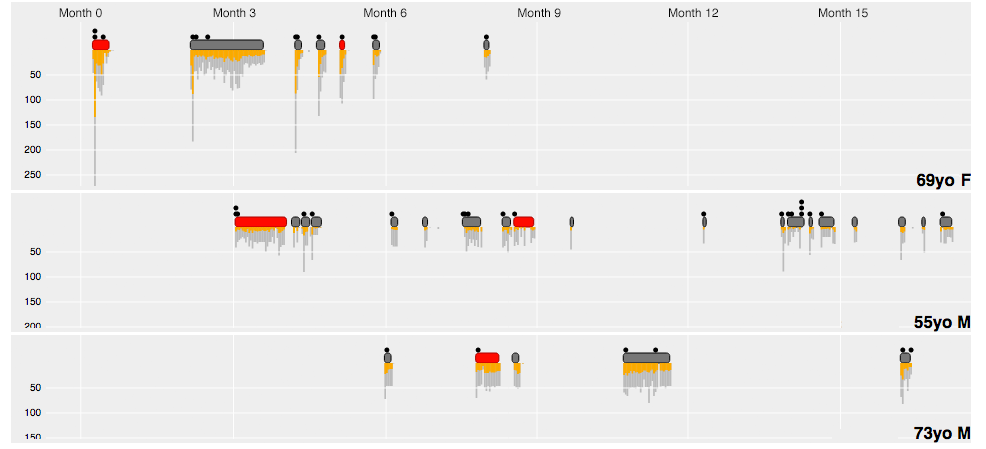
\includegraphics[width=\textwidth]{chap1/pt-timelines-deidentified}               
  \caption[Visualization of EMR data]{\textbf{Visualization of EMR data.} Timelines for two patients generated from EMR data in the Mount Sinai Data Warehouse (original analysis). Patient visits to Mount Sinai are represented as horizontal bars across the top of the timeline, and visits associated with a \textit{C. difficile} infection are highlighted in red.  The number of lab tests ordered per day is represented on the vertical axis, with abnormal results highlighted in orange.  Transfer events are marked by the black dots above the horizontal bars.}
  \label{fig:emr_sample_viz}
\end{figure}
With so many different stakeholders entering EMR data, however, automatically extracting certain facts (e.g., “this patient had the flu last Tuesday”) can be difficult. Nevertheless, high-accuracy methods for extracting infectious phenotypes such as influenza-like illness \sidecite[-1.2cm]{Silva2013}, unclear HIV status,\autocite{Felsen2014} and community-acquired pneumonia\autocite{DeLisle2013} have been demonstrated, and consortia such as eMERGE are standardizing comparison, validation, and deposition of these algorithms into a central repository.\autocite{Pathak2013a}

The marriage of real-time digital clinical information with “omics” technology creates the opportunity to increase the precision of clinical decision-making and challenges us to quickly design and execute bioinformatics analyses. Predictive modeling of infectious disease that incorporates EMR data is still rare, although one recent study generated a social network for hospital acquired infection from EMR data using recorded contacts between patients and caretakers.\autocite{Cusumano-Towner2013} Another found that statistical analysis of EMR data produces risk factors for C. difficile infection that outperform models based only on medically recognized risks.\autocite{Wiens2014} Likely because of the difficulty of integrating data across so many levels, no published studies have yet bridged predictive modeling on EMR data with pathogen genome sequences or other “omics” data from individual patients. Yet, for infectious disease, this is exactly what will fulfill the vision of a rapid-learning health system \autocite{Care2014,Kohane2012} that converts the informational byproducts of healthcare recorded by practitioners into evidence for future decision-making. While EMR data holds details of the clinical process and outcomes, “omics” data ties it back to pathophysiology and the precise strain and host-pathogen interactions present in each patient. Together, they can fuel a “learning engine” that integrates heterogeneous data into new clinical insights, interventions, and therapies. We will discuss how to leverage current bioinformatics software to build such an engine, and how this engine will be able to attack currently insurmountable problems in the field.

\section{The genomic clinical microbiology laboratory}

\newthought{Previous reviews}\autocite{Didelot2012,Koser2012} have proposed that cheap sequencing technology will transform clinical microbiology, while acknowledging technical and informational barriers to adoption. Whole genome sequencing (WGS) via NGS provides ultimate resolution for epidemiological studies of transmission and relatedness, and may soon be cost-effective for routine use.\autocite{Didelot2012,Koser2012} For pathogen identification, however, NGS is unlikely to usurp robotic culturing systems (e.g., Vitek and BD Phoenix) or newer mass spectrometry systems by cost and sensitivity comparisons alone, although it can lower turnaround time for difficult-to-culture organisms and identify novel or rarely-seen pathogens.\autocite{Koser2012,Naccache2015} Since susceptibility or resistance of an organism to drugs is in principle fully encoded in its genetic material \autocite{Didelot2012,Gordon2014}, NGS can also lower turnaround times for drug susceptibility testing of slow-growing organisms, such as M. tuberculosis \autocite{Boehme2010} and HIV-1.\autocite{Ram2015} This strategy should only expand as fuller catalogs of genomic variants that cause drug resistance are compiled for other pathogenic organisms.

\subsection{Leveraging existing bioinformatics tools}

An oft-mentioned hurdle\autocite{Didelot2012,Koser2012} for widespread use of NGS in clinical microbiology is the lack of readily accessible software for converting these data into species identifications, phylogenies, and drug susceptibilities. However, many mature open source bioinformatics solutions for individual components of these problems exist, and connecting these components into a pipeline is therefore a tractable software engineering exercise. Examples for most subtasks are listed in Table \ref{tab:id_bioinf_tools}. As NGS use by clinical microbiology laboratories becomes more commonplace, we might anticipate full-fledged genomic clinical microbiology software packages to become widely available.

\newthought{This expectation} has three foreseeable shortcomings. The first is that current tools are tied to centrally curated repositories of evidence. Although proponents of genomic clinical microbiology often envision encyclopedic databases hosted by international consortia,\autocite{Didelot2012,Koser2012} human curation is expensive and inefficient at scale, and many infectious diseases are locale-specific phenomena. Models based on pooled data may fail to reflect variation between healthcare delivery regions;\autocite{Reis2003,Wiens2014} for instance, a recent fitness model of H3N2 influenza based on international genomic surveillance data creates predictions only at the resolution of clades spanning multiple continents.\autocite{Luksza2014} Since implementation of NGS in a healthcare institution’s microbiology laboratory produces copious sequencing data not easily shared through public databases, institutions should prepare to manage repositories of local evidence and predictive models that work specifically for them. Over time, as data exchange interfaces are developed, institutions could form consortia to generalize analyses, which is a strategy that has successfully increased the power of human genome-wide association studies.\sidecite[-3em]{Gottesman2013,Kohane2012}

\begin{table}[ht]
  \centering
  \small
  \begin{tabular}{l l}
    \toprule
    \textbf{Problem domain} & \textbf{Software or database}\\
    \midrule
    Strain typing &
    \begin{minipage}[t]{5cm}
      \raggedright
      \begin{itemize}[noitemsep]
      \item Multi-Locus Sequence Typing (MLST) database
      \end{itemize}
      \smallskip
    \end{minipage}
    \\
    \textit{De novo} assembly from long reads &
    \begin{minipage}[t]{5cm}
      \raggedright
      \begin{itemize}[noitemsep]
      \item Celera
      \item Hierarchical Genome Assembly Process
      \end{itemize}
    \end{minipage}
    \\
    Species identification &
    \\
    \-\tabindent From clonal sample &
    \begin{minipage}[t]{5cm}
      \raggedright
      \begin{itemize}[noitemsep]
      \item NCBI BLAST
      \item GenBank
      \item Other databases in Table \ref{tab:id_bioinf_dbs}
      \end{itemize}
    \end{minipage}
    \\
    \-\tabindent From non-clonal sample &
    \\
    \-\tabindent\tabindent  Meta-assembly &
    \begin{minipage}[t]{5cm}
      \raggedright
      \begin{itemize}[noitemsep]
      \item AMOS
      \item MIRA
      \item MetaVelvet
      \end{itemize}
      \smallskip
    \end{minipage}
    \\
    \-\tabindent\tabindent Clustering and species annotation &
    \begin{minipage}[t]{5cm}
      \raggedright
      \begin{itemize}[noitemsep]
      \item MEGAN
      \item MG-RAST
      \end{itemize}
      \smallskip
    \end{minipage}
    \\
    Maximum likelihood phylogeny trees &
    \begin{minipage}[t]{5cm}
      \raggedright
      \begin{itemize}[noitemsep]
      \item BEAST
      \item RAxML
      \item ClonalFrame
      \item ClonalOrigin
      \end{itemize}
      \smallskip
    \end{minipage}
    \\
    Whole genome alignment &
    \\
    \-\tabindent For SNP calling &
    \begin{minipage}[t]{5cm}
      \raggedright
      \begin{itemize}[noitemsep]
      \item Mummer
      \item Mugsy
      \item Harvest
      \end{itemize}
      \smallskip
    \end{minipage}
    \\
    \-\tabindent For structural variant calling &
    \begin{minipage}[t]{5cm}
      \raggedright
      \begin{itemize}[noitemsep]
      \item Mauve
      \end{itemize}
      \smallskip
    \end{minipage}
    \\
    Gene annotation &
    \\
    \-\tabindent Bacterial &
    \begin{minipage}[t]{5cm}
      \raggedright
      \begin{itemize}[noitemsep]
      \item Glimmer
      \item RAST
      \item prokka
      \end{itemize}
      \smallskip
    \end{minipage}
    \\
    \-\tabindent Drug resistance in bacteria &
    \begin{minipage}[t]{5cm}
      \raggedright
      \begin{itemize}[noitemsep]
      \item Resfinder
      \item ARG-ANNOT
      \item Mykrobe predictor
      \end{itemize}
      \smallskip
    \end{minipage}
    \\
    \-\tabindent Other &
    \begin{minipage}[t]{5cm}
      \raggedright
      \begin{itemize}[noitemsep]
      \item Influenza Virus Sequence Annotation Tool
      \end{itemize}
      \smallskip
    \end{minipage}
    \\
    \bottomrule
  \end{tabular}
  \caption[Bioinformatics tools for infectious diseases]{Selected published bioinformatics software packages or databases that address specific steps of clinical microbiology tasks using NGS data (this list is not exhaustive). Well-established tools are available for many specific subtasks.}
  \label{tab:id_bioinf_tools}
\end{table}

A second shortcoming is that current pathogen annotation tools primarily make predictions using the simplistic criterion of sequence similarity. Machine learning (ML) algorithms could eventually integrate a wider array of genotypic features extractable from pathogen genomes—variant calls, putative gene and motif annotations, and more—and train holistic models that predict phenotypes. A “top-down,” integrative model predicting limited phenotypes from genotype for Mycoplasma genitalium is available;\autocite{Karr2012} top-down predictions of virulence, however, add the substantial complexity of host interactions. Therefore, genome-wide ML models of virulence have mostly been “bottom-up,” blind to mechanistic knowledge, and oriented toward even smaller-genome pathogens with considerable genomic surveillance data. ML on viral sequence features has predicted more effective antiretroviral combinations for HIV,\autocite{Lengauer2006,Zazzi2012} genetic markers for host selectivity within families of viruses,\autocite{Raj2011a} and optimal strain selection for H3N2 influenza vaccines.\autocite{Luksza2014} In general, given the explosion in available data, significant untapped potential remains for ML-based models that predict virulence, transmissibility, and drug resistance from pathogen genotypes. 

The third shortcoming is that for many common pathogens, these models are still limited by the paucity of clinical metadata linked to sequenced pathogens. Pathogen phenotypes accessible directly from EMRs include prognostic variables, such as length of stay and disposition, and lab results, such as drug susceptibilities. Although lab information systems (LIS) typically do not forward non-clinical results (e.g., growth curves) to EMRs, data exported from the LIS can help define richer phenotypes. For some diseases, EMRs will contain lab results that directly reflect infection severity, e.g., viral load for HCV and HIV patients,\autocite{Norton2014} while other diseases will require more complex criteria.\autocite{DeLisle2013,Klompas2008,Silva2013} Natural language processing of physician notes will facilitate the extraction of complex, high-accuracy clinical phenotypes from the EMR.\autocite{Liao2015,Silva2013} Routine NGS of specimens and EMR data on drugs prescribed and administered will enable ad-hoc studies crossing pathogen genotypes against interventions and outcomes. Richer characterization of particular host-pathogen encounters may be provided by immune and molecular profiling of selected patients, as well as animal experiments that establish individual pathogen genetic associations and molecular mechanisms. Biomarkers derived from such data\autocite{Mejias2014,Querec2009} could enhance predictive models built on a zealous integration of NGS and EMR data.

\newthought{The growth of EMR} phenotype information associated with pathogen genomes will spur a new generation of pathogenicity and risk models based on genomic data. Ideally, these models can drive a “learning engine” that integrates heterogeneous input data from an encounter with an infected patient and predict outcomes for possible interventions. Predictions can be delivered to physicians via clinical decision support systems that complement EMR functions by suggesting relevant actions within a patient’s electronic chart. The closing of the EMR–NGS–EMR loop (Figure \ref{fig:emr_ngs_loop}) should be the ultimate goal of bioinformatics pipelines for genomic clinical microbiology, because this would maximize the utility of data created for clinical encounters, continuously turning yesterday’s observations and outcomes into evidence for tomorrow’s predictions.\sidecite[-2em]{Care2014,Kohane2012}

\begin{figure}[htb]
  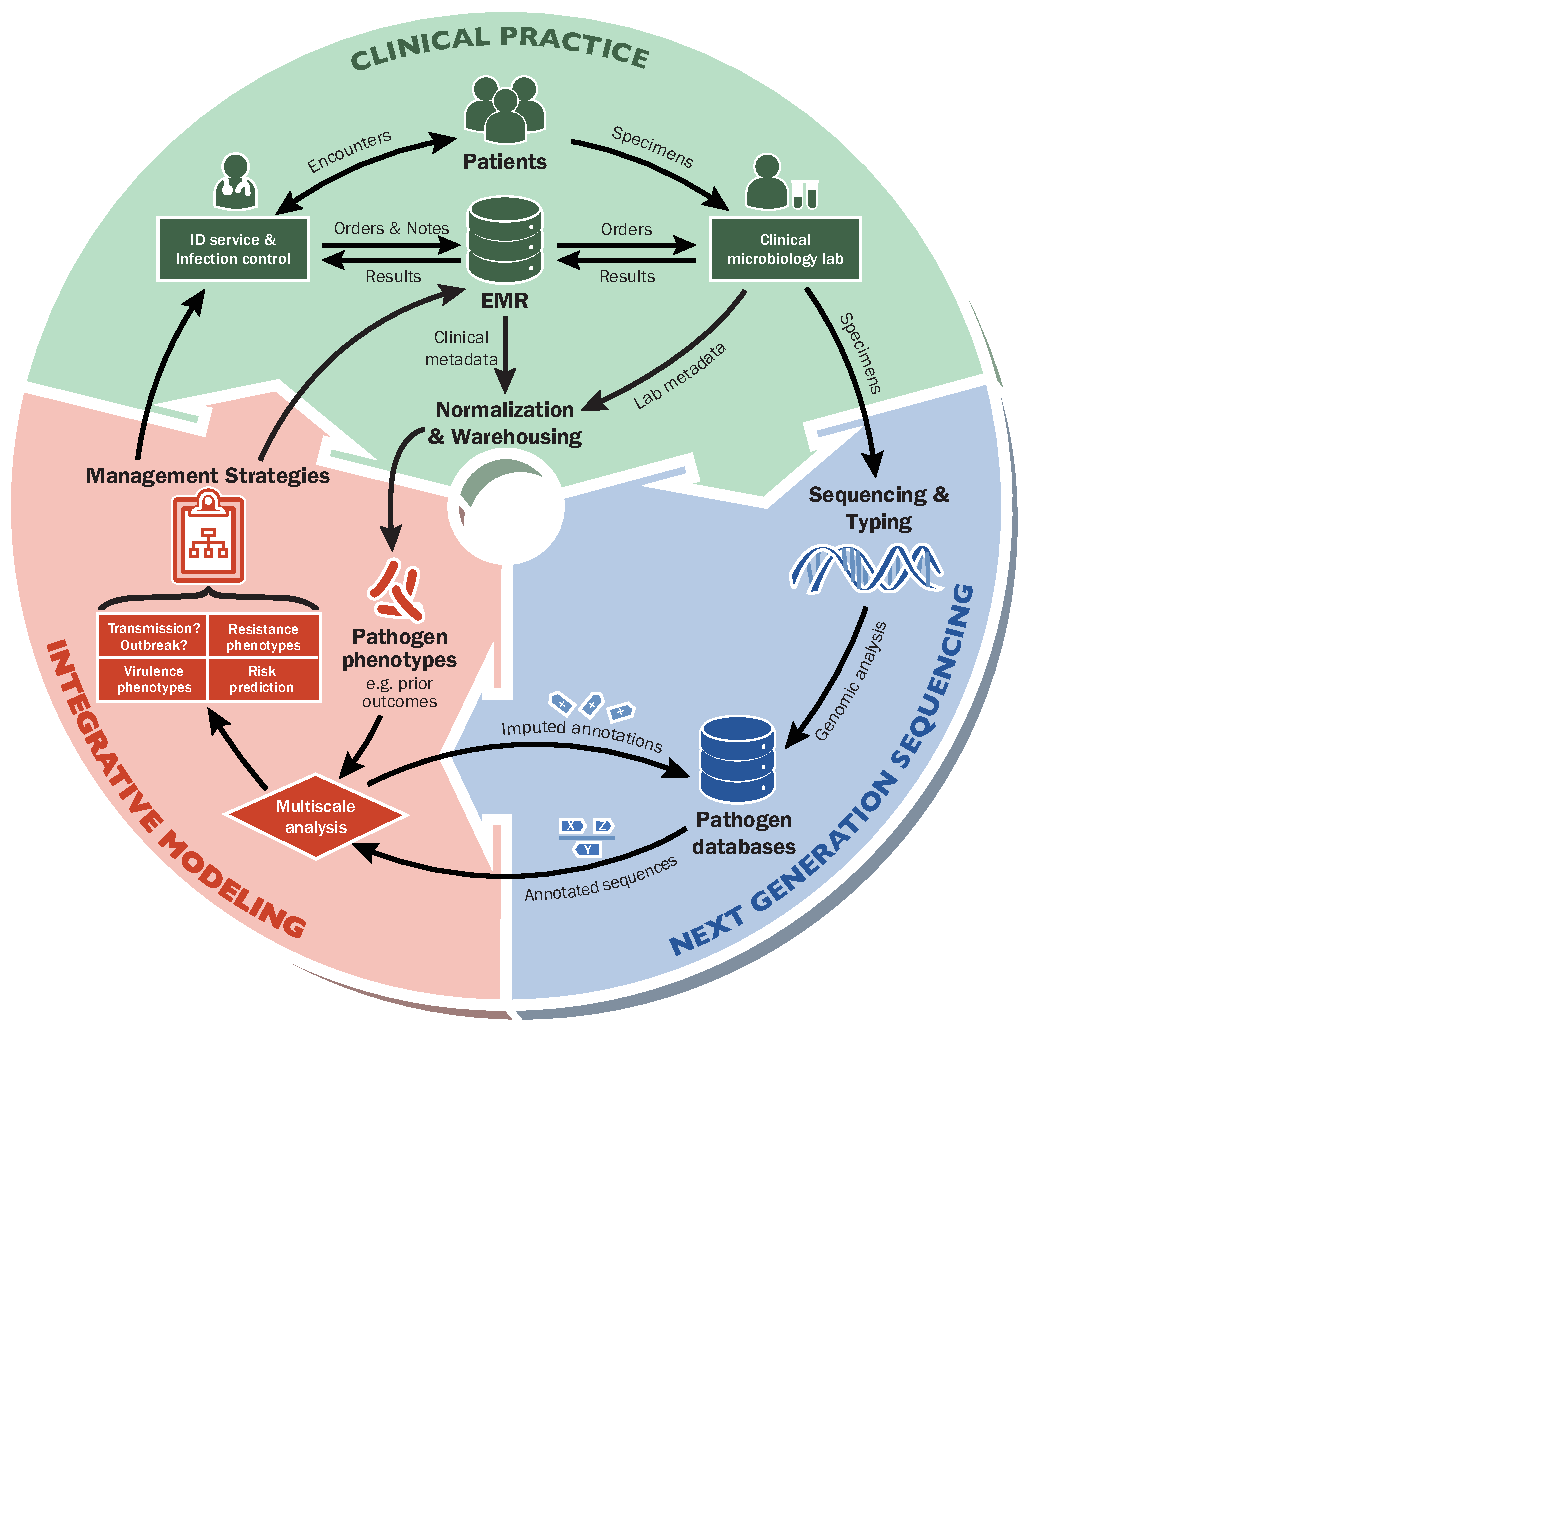
\includegraphics[width=\textwidth]{chap1/emr-ngs_loop_circular}               
  \caption[A learning health system for infectious diseases]{\textbf{A learning health system for infectious diseases.} Next generation sequencing (NGS) technologies now permit routine genomic analysis of clinical microbiology specimens. When integrated with pathogen phenotypes derived from clinical metadata in electronic medical records (EMRs) and laboratory metadata, we can generate predictive models for pathogen transmission, outbreaks, drug resistance, virulence, and risk factors for infection or critical outcomes that are specific to the health system and its patient population. If management strategies are formulated from these predictions and sent to infectious disease (ID) physicians and hospital infection control, a continuous loop of data analysis, application, and model refinement is created.}
  \label{fig:emr_ngs_loop}
\end{figure}

This sounds ambitious, but we can look to analogous software designed as subcomponents of learning healthcare systems to anticipate likely costs and avenues for development. The i2b2 platform\autocite{Kohane2012} and its counterpart SCILHS\autocite{Mandl2014} are vendor-agnostic solutions for extracting and unifying data across EMRs for reuse in cohort design and robust meta-analysis. The eMERGE consortium stimulated the creation of SHARPn for normalization and natural language processing of EMR data\autocite{Rea2012} and CLIPMERGE for automated pharmacogenomics alerts.\autocite{Gottesman2013} For these examples, working software was created after 1-5 years of development with \$100k-\$10M of annual public grant funding.\autocite{Gottesman2013,Kohane2012,Mandl2014,Rea2012} If the aforementioned open-source software is leveraged, an equal scale of public funding and collaboration among academic medical centers could make similar strides toward the proposal in Figure \ref{fig:emr_ngs_loop}. A modular framework allowed i2b2 to expand in scope organically after initial release,\autocite{Kohane2012,Mandl2014} suggesting that successful strategies should first aim for simple but clinically useful tasks such as identifying species and transmissions while anticipating the addition of more complex analyses via plugins and community contributions. In short, a reasonable investment in scrupulous software engineering could produce the seeds of a learning health system for infectious disease within the decade.

\section{Beyond genomic data}

\newthought{While NGS rapidly} moves toward routine use by clinical microbiology laboratories where it can be integrated with EMR data, other advances in data collection on infectious diseases create significant opportunities for predictive modeling that may eventually impact clinical practice. We now review these additional sources of data.

\subsection{Immune profiling}

Host response to infection is not merely the result of single gene modulations or amplification of specific cell types, but rather consists of complex interacting networks of RNA transcription, protein signaling and metabolism that impact cellular, tissue, and whole organism behaviors. The nature of the modulations that are specific to the host’s particular system relative to the state of the system at the time of infection ultimately determines risk and severity of disease. Recent studies have used “omics” scale experimental techniques to provide groundbreaking insight into immune responses, ranging from classification of acute respiratory infections in children\autocite{Mejias2014} and predicting immunogenicity of a vaccine\autocite{Querec2009,Furman2013} to characterizing effects of aging that gradually decrease vaccine efficacy.\autocite{Poland2014}

In each of these studies, researchers took an unbiased, hypothesis-free approach to their design and observed as many properties of the immune system as was experimentally feasible before, during, and after a perturbation, such as vaccine administration. Such properties include cytokine levels as measured by Luminex assays, global changes in gene expression within various leukocyte populations as measured by RNA-seq or microarrays, and changes in cell populations with various surface markers as observed by flow and mass cytometry. With sufficient sample size, patterns of biomarkers can be linked to various clinical outcomes, e.g., the host becoming immunogenic to an antigen. These biomarkers can then be investigated further for their functional role or used in new assays for point-of-care diagnosis. For common presenting conditions, like acute febrile illness, where current diagnostic methods poorly distinguish between bacterial and viral disease, this capability would allow prompt selection of the most appropriate therapy.\autocite{Mejias2014} For diseases like dengue that do not have accurate markers of immunization, these markers will be essential for development of a successful vaccine.\autocite{Mahalingam2013}

\subsection{The internet}

\begin{figure}[htb]
  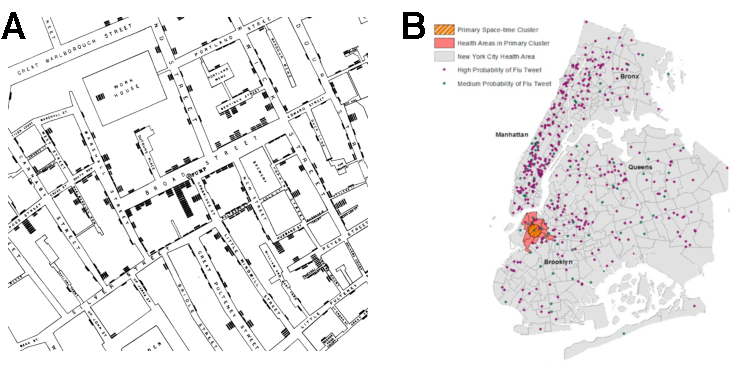
\includegraphics[width=\textwidth]{chap1/snow_and_new_combined}               
  \caption[Geospatial analysis, then and now]{\textbf{Geospatial analysis, then and now}. A, Excerpt from a map published by John Snow in 1855 depicting a cluster of cholera cases around a water pump on Broad Street in London, England. B, Retrospective analysis of geocoded tweets in New York City classified by the probability of representing actual influenza cases during the 2012-2013 flu season, from \textcite{Nagar2014}. The primary outbreak cluster was determined to be in Northern Brooklyn.}
  \label{fig:snow_and_new_combined}
\end{figure}

Patients can now be associated with a trove of digitized information that can be mined to better understand infectious disease. Frequent social contacts are often captured in address books, email inboxes, and social networks like Facebook. Patients discuss symptoms online, which have been captured from search engine queries\autocite{Ginsberg2009} or public Twitter streams to find probable cases of pertussis, whooping cough, and influenza,\autocite{Nagel2013} although these studies have known limitations.\autocite{Lazer2014} Often this data is attached to geospatial information, which can be used to construct spatiotemporal models of the disease that reveal clusters and the directionality  of spread within a city environment,\autocite{Nagar2014} providing in real time the same type of analysis that 19th century anesthesiologist John Snow meticulously compiled to identify a London water pump handle as the source of a cholera outbreak (see Figure \ref{fig:snow_and_new_combined}).\autocite{Buechner2004,Snow1855} Global human movement patterns are also captured in air travel network usage data, which has previously been combined with genomic surveillance data to predict transmission dynamics of H3N2 influenza.\autocite{Lemey2014} Unifying such diverse data in clinically relevant models with actionable outputs remains a significant challenge. On the other hand, the advent of cloud computing and open-source data science platforms like Apache Hadoop, used by Facebook and Walmart to model complex consumer behavior, suggests that algorithms for large, heterogeneous datasets will become increasingly accessible to healthcare providers and life sciences researchers.\autocite{Mohammed2014}

\section{Impact on clinical management}

\newthought{Three potential applications} of a new learning healthcare system for infectious diseases could address some of the most urgent global problems in infectious disease. One problem is rising antimicrobial resistance, which the World Health Organization names one of the three greatest threats to human health.\autocite{Policy2010} Care providers overusing antimicrobials and fomenting resistance in subclinical carriers are partly to blame, with recent studies estimating the fraction of misuse to be between quarter to half of all treatments.\autocite{McKellar2014} Multidrug resistance increases the morbidity and mortality of healthcare-acquired infections (HAIs), which have an incidence of 1.7 million cases per year in the US and an estimated annual cost of more than \$30 billion \autocite{Scott2009} that dwarfs the likely cost of any informatics-based preventative efforts. The sobering threat of extensively drug-resistant community-circulating organisms, some of which have therapeutic failure rates of 25-29\%,\autocite{Hirsch2010} alters the risk analysis for hospital procedures once considered routine and calls for comprehensive new strategies for management.

\subsection{Identifying high-risk patients for HAI}

Infection control for HAIs depends on identifying high-risk patients and applying isolation precautions or reducing known risk factors during their hospital course. For C. difficile infection (CDI), the most frequently reported nosocomial infection in the US, many questions about how infections are acquired and managing at-risk patients remain.\autocite{Leffler2015} The prevailing notion that infections are mostly transmitted person-to-person within hospitals \autocite{Cohen2010} conflicts with recent NGS evidence that sources of infection are more diverse,\autocite{Eyre2013} suggesting a greater role for asymptomatic colonized patients and environmental sources.

Each healthcare system represents a unique milieu of person-to-person contact networks, contaminated surfaces, microbiomes, and asymptomatic colonization that contributes to the risk of CDI. EMR and NGS data can prove or disprove transmission between patients and unlock the secrets of modifiable risk factors in this chaotic environment. ML algorithms predicting individual risk of CDI for a large hospital performed better (area under receiver operator curve, AUC=0.81) when operating on >10,000 unconstrained EMR variables rather than curated variables for known risk factors.\autocite{Wiens2014} Similar ML models based on EMR data between 2009-2014 for The Mount Sinai Hospital in New York City, encompassing 192,000 patients and 1,366 CDI diagnoses, show equal performance (AUC=0.80) and draw out associations not typically published for CDI. These may be unique to Mount Sinai’s environment and include respiratory failure (odds ratio OR=8.3, 95\% confidence interval 6.6-10.3), nutritional irregularity (OR=6.6, 4.7-8.6), and pancytopenia (OR=4.4, 3.1-5.5) (Timothy O’Donnell, personal communication).

A model-based decision support system would screen patients with higher CDI or asymptomatic colonization likelihood and allow earlier diagnosis and intervention. NGS-confirmed transmission events and interactions between people and equipment seen in the EMR and other data could extend this basic model to highlight common factors behind verified transmission and inform empirical, real-time modifications of infection control policy. Cross-sectional analysis by NGS-derived phenotypes and risk factors in the EMR would facilitate more precise clinical decision-making, for instance, whether shortening patient time in intensive care units or decreasing use of provocative antibiotics would be more preventative within the local milieu.  Short of a clinical trial that is probably infeasible to conduct, much less replicate across institutions, there is scant evidence for making these decisions at present, so a localized quantitative model can only help.

\subsection{Earlier detection of outbreaks inside and outside the hospital}

Current infection control software suites like VigiLanz Dynamic Monitoring Suite and TheraDoc Infection Control Assistant primarily issue outbreak alerts based on infection frequency thresholds. This could be rendered obsolete by routine NGS of clinical microbiology specimens, which determines with great precision whether a transmission event has occurred.\autocite{Didelot2012,Koser2012} A software system with access to EMR and other hospital data could automatically search elements common between verified transmission cases (caregivers, equipment, or rooms) and alert staff to inspect these elements before they produce enough transmissions to trigger a frequency threshold alert. Given enough historical data, NGS could also help hospitals differentiate community- from hospital-acquired infections and thereby refine metrics used to evaluate infection control policies.

An active effort to sample the environment inside and outside the hospital could further extend the reach of this surveillance. Within the hospital, “problem spots” identified by earlier investigations could be resampled regularly via NGS to re-evaluate the efficacy of infection control measures. The hospital also samples the pathogen ecosystem of the local population. Hospitals already report diagnoses of highly transmissible and dangerous infections to government authorities, and sharing NGS data for these cases would permit real-time assessment of where pathogens are coming from, how they are evolving, and where populations naïve to a pathogen are located. Current mapping and surveillance efforts \autocite{Brownstein2008} would be vastly enhanced by rich phylogenetic information, allowing outbreaks across disparate regions to be linked.\autocite{Chin2011,McAdam2012,Rasko2011} Fine-grained, real-time tracking of infectious disease spread would better inform doctors diagnosing and treating new patients, field agents tracking cases and contacts, and health policymakers seeking preventive population measures.

\subsection{Antimicrobial stewardship}

Decision support systems for empirical antibiotic therapy have been investigated for decades,\autocite{Leibovici1997} but with the prevalence of antimicrobial resistance skyrocketing, the urgency to implement systems that specifically encourage restraint with antibiotics has increased.\autocite{Wagner2014} Selective reporting is a common strategy that directs providers toward optimal therapies simply by omitting names of inappropriate drugs in susceptibility reports.\autocite{Doern2013} A more aggressive strategy pushes EMR alerts whenever physicians prescribe antibiotic treatment inconsistent with best practices.\autocite{Kullar2013}

These solutions ignore the power of the EMR to provide evidence that justifies or improves the antimicrobial stewardship interventions. For instance, although it is well accepted that antibiotic overuse increases the prevalence of resistance, current antimicrobial stewardship programs have demonstrated neither effects on patient outcomes nor even that decreased antibiotic treatment leads to decreased antibiotic resistance.\autocite{Wagner2014} By integrating NGS and EMR data, these hypotheses could be investigated in minute detail within large patient cohorts. NGS can reveal and enumerate the genetic mechanisms of resistance circulating through a health system. By tracing the recurrence of pathogens in the local community, an NGS-equipped health system can determine whether patients receiving antibiotics have generated and transmitted drug-resistant mutants. Specific drug regimens can be correlated with the development of particular resistance mutations. Conversely, given enough longitudinal data, the efforts of an antimicrobial stewardship program can be validated by observing decreased emergence of resistance mutations to drugs prescribed more conservatively.

\section{Conclusions}

\newthought{Routine access} to pathogen genomic data will transform our ability to manage infections, but only if we can integrate this information with clinical and other data to power predictive models for critical outcomes. Assuming that the hurdles of cost, accuracy, and turnaround time can be addressed, which is likely given current trends, NGS will soon become a standard clinical microbiology procedure. The unprecedented specificity of this data will in the near term allow reconstruction of transmission networks inside and outside of hospitals. In the far term, having rich clinical data linked to pathogen genotypes will permit predictions of prognosis, virulence, and drug susceptibility for active infections once NGS data is available. Incorporating these capabilities into a new clinical workflow that actively refines predictive models by adjusting to new data (Figure \ref{fig:emr_ngs_loop}) should improve case management, risk prediction for HAIs, detection of outbreaks, and antimicrobial stewardship. The missing link in this transformation, and the goal for bringing it to fruition, is software that leverages best-of-breed existing tools, incorporates all relevant heterogeneous datatypes, builds on electronic phenotyping algorithms to scrub low-accuracy EMR data, and validates against gold standard clinical case review.
Healthcare institutions and researchers should recognize that a potent combination of NGS and EMR data will transform infectious disease management. The threats posed by multidrug resistance and healthcare associated infections demand a revolution in management strategy. Predictive modeling grounded in rich, diverse molecular and clinical data will dramatically increase the precision of care and help hold these threats at bay.

\section*{Notes}

A shortened version of this chapter was published in \textit{Clinical Infectious Diseases}.\autocite{Pak2015}

\subsection{Acknowledgements}

We thank Deena Altman and Shirish Huprikar for critical suggestions on the manuscript.

\subsection{Financial support}

The authors were supported by the Icahn Institute for Genomics and Multiscale Biology at Mount Sinai.

\subsection{Potential conflicts of interest}
We certify no potential conflicts of interest.
